\documentclass{article}

\usepackage{amsthm, amssymb, amsfonts}
\usepackage[margin=1in]{geometry}
\usepackage{graphicx}
\usepackage{epstopdf}
\usepackage{comment}
\usepackage{tabto}
\usepackage{mathrsfs}
\usepackage{stmaryrd}
\usepackage{relsize}
\usepackage{latexsym}
\usepackage{float}


\begin{document}

\title{GridStat on DETER Proposal}

\author{Ryan C. Goodfellow \\
	Information Sciences Institute \\
	Marina Del Rey, CA \\
	\texttt{rgoodfel@isi.edu}}

\date{\today}

\newtheorem{thm}{Theorem}[section]
\newtheorem{cor}[thm]{Corollary}
\newtheorem{lem}[thm]{Lemma}

\theoremstyle{remark}
\newtheorem{rem}[thm]{Remark}
%\newtheorem{proof}[thm]{Proof}

\theoremstyle{definition}
\newtheorem{defn}[thm]{Definition}
\newtheorem{exmp}[thm]{Example}
\newtheorem{prop}[thm]{Proposition}

\newtheoremstyle{axiom}{}{}{\itshape}{}{\bfseries}{}{.5em}{\thmnote{Axiom #3 }}
\theoremstyle{axiom}
\newtheorem*{axiom}{Theorem}


\maketitle

\section{Background}

\subsection{The Power System}
In the modern world, we have come to enjoy electric power as a commodity for many 
decades now.  The system that provides us with electricity, the electric power grid, 
began in 1882 when Thomas Edison launched the Pearl Street Station Power Plant. This 
first power grid provided electricity for several city blocks in New York city.  Fast 
forward to today, the power grids that we have are so vast and interconnected that they 
commonly transcend our most significant political borders and are considered as a single 
transcontinental system.  There have obviously been many engineering feats accomplished 
to bring us from the Pearl Street grid to what we see today.  Electricity is a tricky 
commodity in that it can not be stored in significant capacities.  This means that 
supply must always exactly meet demand in an electric power system.  Electrical 
engineers have been able to achieve this in electric power systems by constructing 
instrumentation and control systems.  In the early days this was relatively simple.  
System engineers would decide on some voltage level they wanted to keep the system at.  

The ratio of the actual system voltage to this decided operational voltage is called the 
per unit voltage of the electrical system.  If the per unit voltage in the system 
started to ascend away from 1, then there was too much supply (generation) of 
electricity in the system.  Dually, if the per unit voltage in the system started to 
descend away form 1 then there was not enough supply to meet demand (load).  This is 
all based on the fundamental fact that ${P = VI \equiv V = P/I}$ where P is power, I 
is current and V is voltage.  If we want voltage stability at some target per unit 
quantity, in the face of fluctuating current demanded by the users of the system then 
we must control power generation in response to demand.  On this basis, systems 
engineers could keep track of per unit voltages at carefully selected locations 
within a system, send these quantities to controllers at generation stations and 
keep the supply demand problem in check.  As such systems have become more complex 
over the years we have given them a special name, \emph{supervisory control and 
data acquisition} (SCADA) systems. \\

SCADA systems are only a part of the engineering makes electric power systems 
possible.  Another significant area of engineering within the power system is what 
are known as \emph{protection automation control} (PAC) systems.  These systems protect 
the physical power system and its users from more stochastic sources of instability 
such as lighting storms, falling trees and backhoes.  When lightning strikes a power 
line, a tree falls through one, or a backhoe digs through one, the devices that comprise 
PAC systems can detect the resulting electrical effect and take corrective action to 
prevent damage of equipment or injury to users.  The canonical example of a simple PAC 
system is a protective relay and a breaker.  A protective relay instrumenting a 
transmission line can detect when a tree falls through a transmission line by the 
electrical effect it has.  Say the result of the tree falling on the line is the line 
falling to the ground and energizing the earth.  This is known as a line to ground fault 
and will cause current in the line to shoot up and voltage to dip down, a condition 
called overcurrent.  The relay on the transmission line can detect this condition.  
In response it opens a breaker, disconnecting the faulted line from it's power source.  
If this relay were not present in such a situation, either a transformer connected to 
the line could burn out in a violent fashion due to extreme currents or in the worse 
case the generator supplying the line could become overloaded and break down.  The cost 
of the PAC system is disproportionately low to the potential damage caused in its 
absence.  Without PAC systems stable operation of the electric power system would be 
impossible. \\

Together, SCADA and PAC systems provide for most of the stability and reliability that 
is seen in todays electric power systems.  The evolution known as the 'Smart Grid' 
happening today is the process by which pure electrical and electromechanical systems 
within the SCADA and PAC realm are being replaced by digital microprocessor based 
devices interconnected by computer networks.  With this movement comes a huge potential 
for advancement in power systems engineering.  Realization of this potential, however, 
is not without cost.  In the context of the power system, that cost is complexity.  
The fact that electric power is a commodity in modern economies is the result of over 
a century of interplay between the theory and practice of engineering electric power 
systems.  Integrating microprocessor based devices operating over computer networks 
into the systems responsible ensuring stability and protection \emph{increases the 
complexity} of the system as a whole.  This engineering space is coming to be known as 
cyber-physical systems engineering.  In the limit, the physical portion of a 
cyber-physical system stops at physical instrumentation and actuation and the cyber 
portion does everything else.  To flesh this out a bit in context, for the power 
system, the only physical components of PAC and SCADA systems will be the devices 
instrumenting conducting equipment and the devices actuating breakers, switchgear, 
governors and other mechanical devices.  Everything else will be handled by the cyber 
portion of they system.  The motivation for this is programability.  Unlike an 
electromechanical device, computers are arbitrarily programmable and thus flexible. 
A prime example of this is the modern digital relay. In the past, an electromechanical 
relay could detect overcurrent and operate a breaker, but that was about it.  
Electromechanical relays could not coordinate with one another to protect a 
transmission line \emph{system}, or provide detailed instrumentation information about 
electrical events that induced control actions like todays protective relays.  This 
xample extends to many other components in the power system.  Distributed generation 
such as wind and solar energy, which can only probabilistically provide power is a 
rising trend in many power systems.  The stochastic nature of these sources can 
adversely affect the stability of the system. As more distributed generation sources 
proliferate into our power system, the need for programable distributed control will 
only be amplified. Digital relays operating over computer networks making possible 
distributed coordination within PAC systems was the first step.  The state-of-the art 
in coordination and control algorithms realized in this realm today are quite localized 
and very rudimentary.  An example of this would be two protective relays at either end 
of a transmission line agreeing on the fact that there is a significant voltage 
differential across the line and that protective action must be taken.  Distributed 
control (for the PAC realm) does not extend far beyond this level of complexity, in 
most cases due to the fact that the communication systems that exist can not support 
the desired algorithm.  This is where we can bring field of \emph{distributed computing} 
to the power system.\\

The integration of distributed systems into critical sections of the electric power 
system is quite possibly the grandest challenge that has ever faced coordinated 
distributed computing, in theory and practice.  The magnitude of the time and space 
requirements are unprecedented.  The power system runs at a rate of 60 Hz and flows 
at the speed of light, any distributed system operating in this environment must run 
at a scalar multiple of the rate and keep up with the flow.  The size in space of the 
power system spans entire continents with digital participants at least on the order of 
10$^{5}$ today and accelerating toward tomorrow. \\

\subsection{GridStat}
The power system is a rate based synchronous system. The control systems that operate 
in local and wide areas of the power grid instrument this rate based system and 
maintain its stability by performing asynchronous discrete control actions.  Control 
systems operating in the wide area require rate based data delivery at a defined scalar 
multiple of the power system operational rate of 60 Hz.  Over a decade of research has
 gone into the GridStat data delivery system to provide wide-area rate-based data 
delivery with the strong quality of service (QoS) guarantees demanded by control 
systems.  GridStat is implemented as a data-centric publish/subscribe middleware.  
When subscriptions are made, GridStat guarantees that a data path will be constructed
 between the publisher and the subscriber that ensures the data rate and latency 
requirements of the subscription.  GridStat also ensures that data paths from publishers 
to subscribers are fault tolerant through routing algorithms that create disjoint 
optimal paths between publishers and subscribers.  By virtue of being data-centric, 
publishers are not aware of subscribers and subscribers are not aware of publishers. 
 Each participant is simply aware of the data it is providing or consuming, e.g. the 
data itself decouples its producers and consumers.  The GridStat data delivery system 
exists as a few logical entities; publishers, subscribers, the data plane and the 
management plane. Publishers and subscribers publish and subscribe data respectively, 
the data and management planes work cooperatively between publishers and subscribers 
to get publication data to subscribers at the rate they require it.  The data plane is 
a graph of entities called forwarding engines that forward data from publishers to 
subscribers.  The management plane consists of QoS-Brokers that facilitate subscription 
requests by constructing paths in the data plane between publishers and subscribers 
that can guarantee the requested data-rate.  Consider the figure below. \\

\begin{figure}[h]
\begin{center}
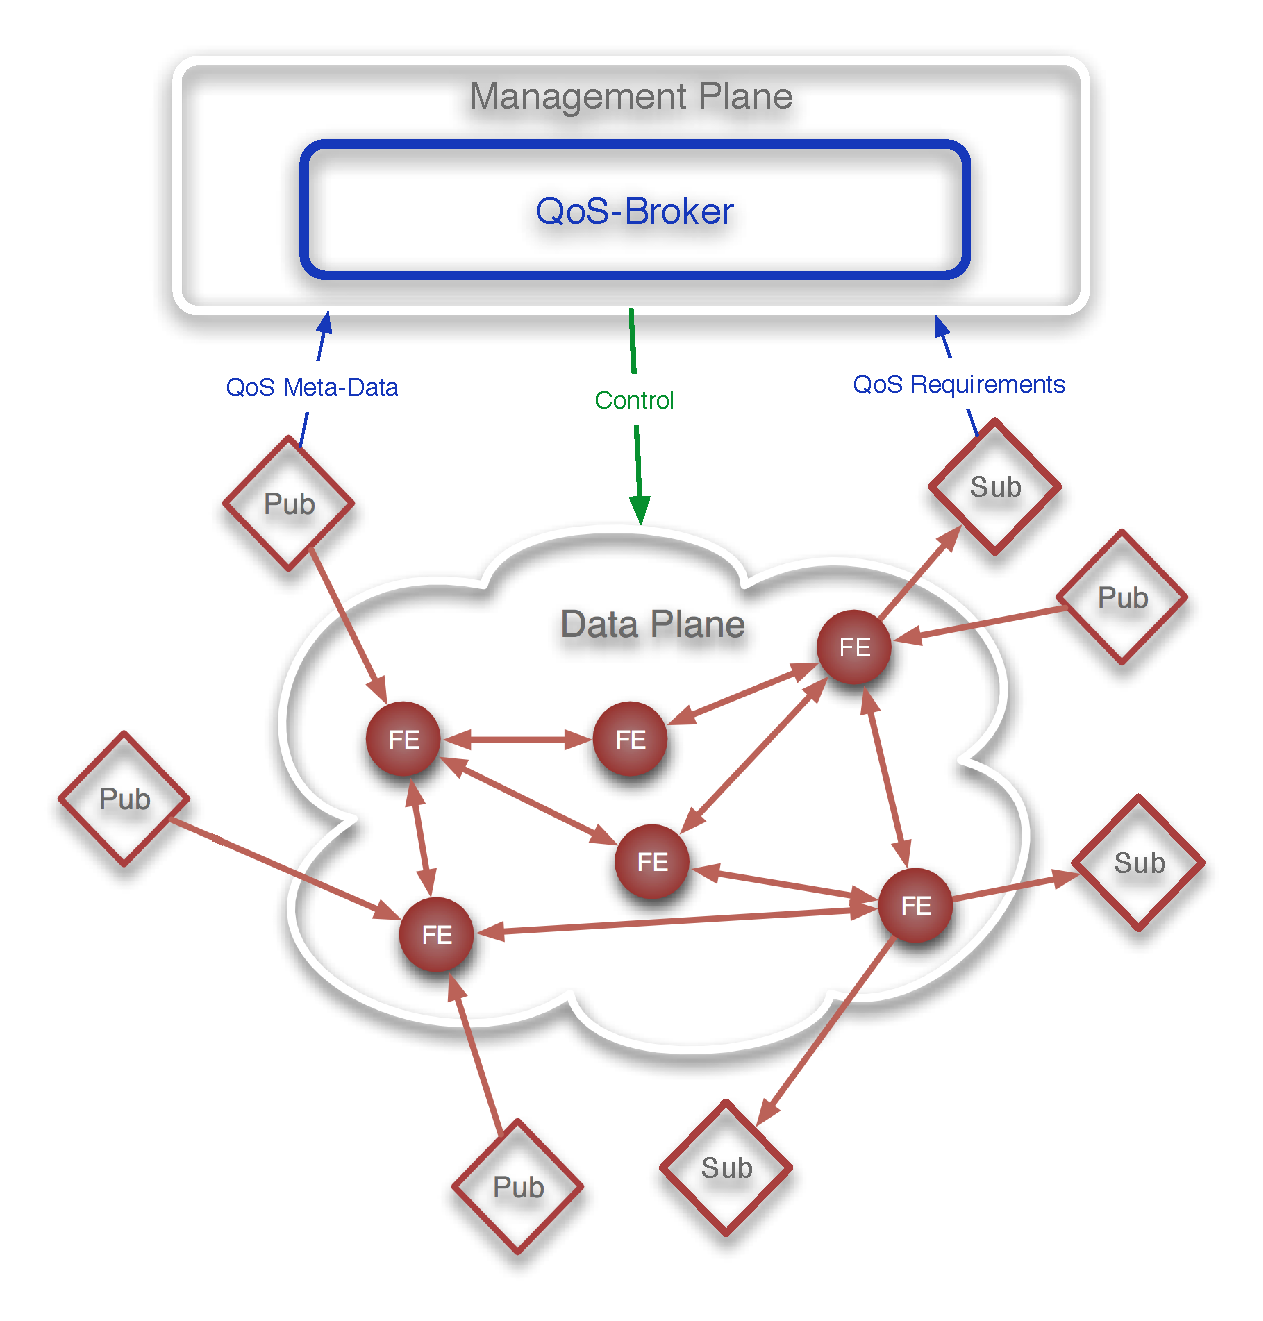
\includegraphics[scale=0.51]{GridStatSimple.eps}
\end{center}
\caption{Simple GridStat System}
\end{figure}

Here we have a simple GridStat system with all of the entities just described.  
Let's walk through the basics of how the system works.  When a publisher comes online
 it sends QoS meta-data to its QoS broker.  This is basically making the QoS broker
 aware of both the presence of the data variable available for subscription and the 
maximum rate at which it may be provided.  When a subscriber requests a variable at a 
given rate, it is the management plane's responsibility to construct a path through the 
data plane that gets the data from the publisher providing the variable to the
 subscriber requesting it, at the rate which the subscriber has requested it. 
 If this is not possible then the management plane will reject the subscription
 request.  The management plane will construct data paths in such a way that publishers
 and forwarding engines are only moving data at the minimum rate as dictated by 
subscriptions. For example, if a publisher is advertising a variable available at 
1440 Hz, but the highest rate subscription for that request is at 30 Hz, than that
variable will only move through the system at a maximum rate of 30 Hz.  
This concept also extends to path junctions in the data plane, if a forwarding 
engine is multiplexing a variable path downstream, it will only provide each outgoing 
path with the minimum required data-rate.  Thus, if a forwarding engine is receiving
 a variable stream at 60 Hz and is forwarding to 2 participants at 60 Hz and 25 Hz, 
then for the 25 Hz path, the incoming rate is down sampled to the required rate. This 
significantly improves the scalability of the system relative to common practices seen 
today in the power system such as 'wide-area ethernet' where all signals are sent at 
the highest rate possible. Notice that in this system there is only a single QoS-Broker.
  What this means is that this QoS-Broker 'owns' the entire data plane and all 
publications and subscriptions must go through this broker.  Now consider the case 
where we have two QoS-Brokers.


\begin{figure}[h]
\begin{center}
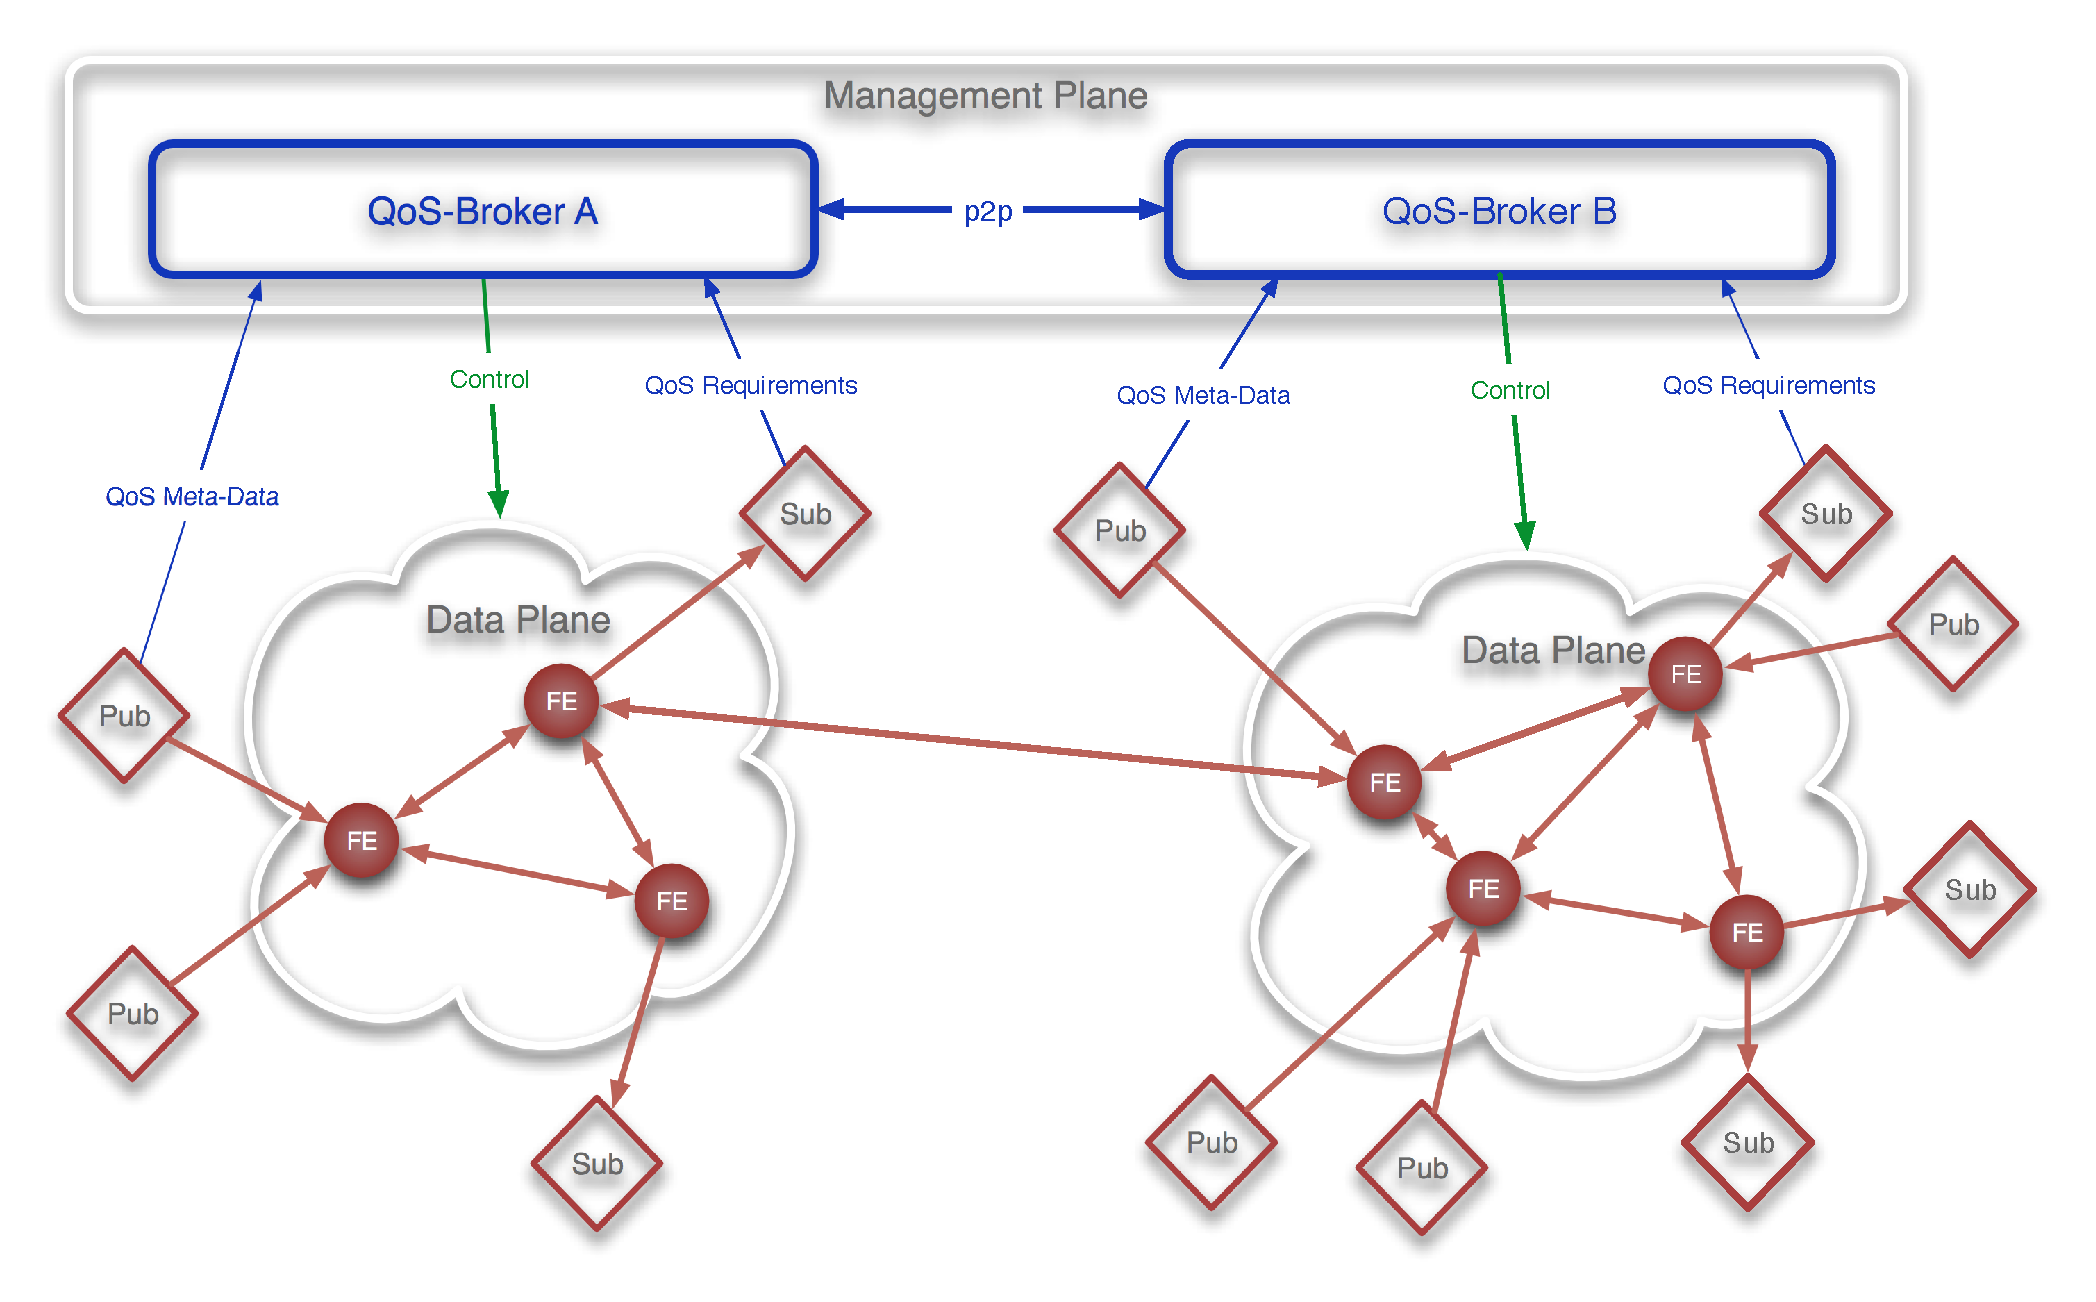
\includegraphics[scale=0.51]{GridStat2Broker.eps}
\end{center}
\caption{Two Broker GridStat System}
\end{figure}

The situation here is the same as the single broker except for the case when a 
subscriber in QoS-Broker B requests a subscription to data from a publisher in
 QoS-Broker A.  In this case, each QoS-Broker must create the paths within its own
 data plane and they also must agree on a path between their respective data planes. 
 There are many good reasons for partitioning the system in to multiple brokers. 
 In terms of performance and non-functional requirements; it can reduce the
 computational load experienced by the brokers from subscription requests, single points
 of failure for the entire system are at least reduced and individual logical brokers
 can be easily replicated for fault tolerance reasons.  In terms of functional 
requirements, it allows for multiple participants in a GridStat system to cooperate
 in flexible and tightly managed ways.  If the above diagram represented a transmission
 company (TRANSCO) and a distribution company (DISTCO), the TRANSCO certainly only wants
 to share certain information with the DISTCO and vice versa.  Additionally each entity 
would want to control the number of external subscriptions and the rates at which those
 subscriptions are made available.  Essentially the organizations are encapsulating the
 data within their network and protecting that network form being overloaded by external 
sources. In a peer-to-peer system of QoS-Brokers, this type of cooperation and control
 becomes possible. \\

Recent unfortunate history, with several major power-system black-outs shows us why
 wide-area situational awareness is a essential for maintaining system stability.  
This task requires robust real-time communication that transcends many corporate 
domains.  GridStat aims to fill this role.  


\section{GridStat and DETER}

In this section I will outline my proposal for deploying and experimenting with GridStat
 on the DETER testbed.  The long-term goal of this work is to engineer a testbed 
environment within DETER for experimentation in wide-area communication and control
 for power systems.  This problem space can be partitioned into three almost mutually 
exclusive areas of research and development;  power system simulation, control system 
design and communication system design.  Power system simulation exists on its own with 
no real dependency on either the communication or control system.  The control system
 obviously must have hooks into the simulated power system to instrument signals and 
control mechanical actuation within the simulation, but that is about the extent of 
the interaction between the two.  The complexity of power system simulators is very 
high, and unfortunately I do not know of any simulation systems that can take advantage 
of the scalability offered by cluster computing environments.  Power system simulators 
today are designed for single processor systems, and consequentially, the answer to 
simulating a larger system is buying a faster processor (which is obviously a very 
limiting scalability factor).  There are some simulators on the market that claim to 
support distributed computation, however, whether these systems have been proven with 
real large power systems is yet to be determined.  Even if these simulators are ready 
for prime time, the immensely complex models that exist for real, large power systems 
must be translated into a format the distributed simulator can understand which itself 
is a substantial undertaking.  In moving forward with this research, I strongly believe 
that monolithic simulator systems are \emph{not} the answer. Thus research in this area 
will be necessary, however, because this area can be nicely decoupled from communication,
 which is my primary research area, it can wait.  \\


The underlying requirements that motivated the original development of GridStat are 
from the power system, but are not exclusive to that domain.  The essentials of the 
system are wide-area rate-based communication with real time requirements that span 
multiple domains of ownership.  With this in mind, we can somewhat decouple GridStat 
from the power system and leverage DETER for experimentation and research of GridStat
 itself as a communication system that facilitates these goals.  This is what I plan
 to focus on for the first phase of the research.  However, keeping in mind the long 
term goals of this research, certain aspects will be influenced by the power system. 
 This brings me to the deployment strategy for GridStat on DETER. \\

\subsection {Deployment Topology}


%%%%%%%%%%%%%%%%%%%%%%%%%%%%%%%%%%%%%%%%%%%%%%%
Several years ago, I lead a joint project between Washington State University (WSU), 
Bonneville Power Administration (BPA) and Schweitzer Engineering Laboratories (SEL). 
 The goal of this project was building a GIS visualization system that facilitated the 
wide-area situational awareness made possible by synchrophasor data produced by SEL
 phasor measurement units (PMU).  From this project I have gained a good working 
knowledge, as well as the actual data that describes the topology of the transmission
 system in the northwest region of the U.S.  What this can provide for my research here,
 is a base GridStat system topology to start with that reflects a real world power 
system.  Figure 3 shows a map of what this power transmission system looks like.  What
 the map shows is blue dots representing substations and yellow lines representing 
transmission lines.  In all there are 521 substations and 614 transmission lines owned 
by 117 different organizations.  What this provides for us with the GridStat deployment 
on DETER is a nice reference model.  We have 117 organizations, so we have at least 117 
QoS-Brokers.  There are far more organizations that own substations than own 
transmission lines.  What this identifies is the set of substations at which the 
transmission system is feeding a distribution system or is being fed by a generation 
station. \\

\begin{figure}[h]
\begin{center}
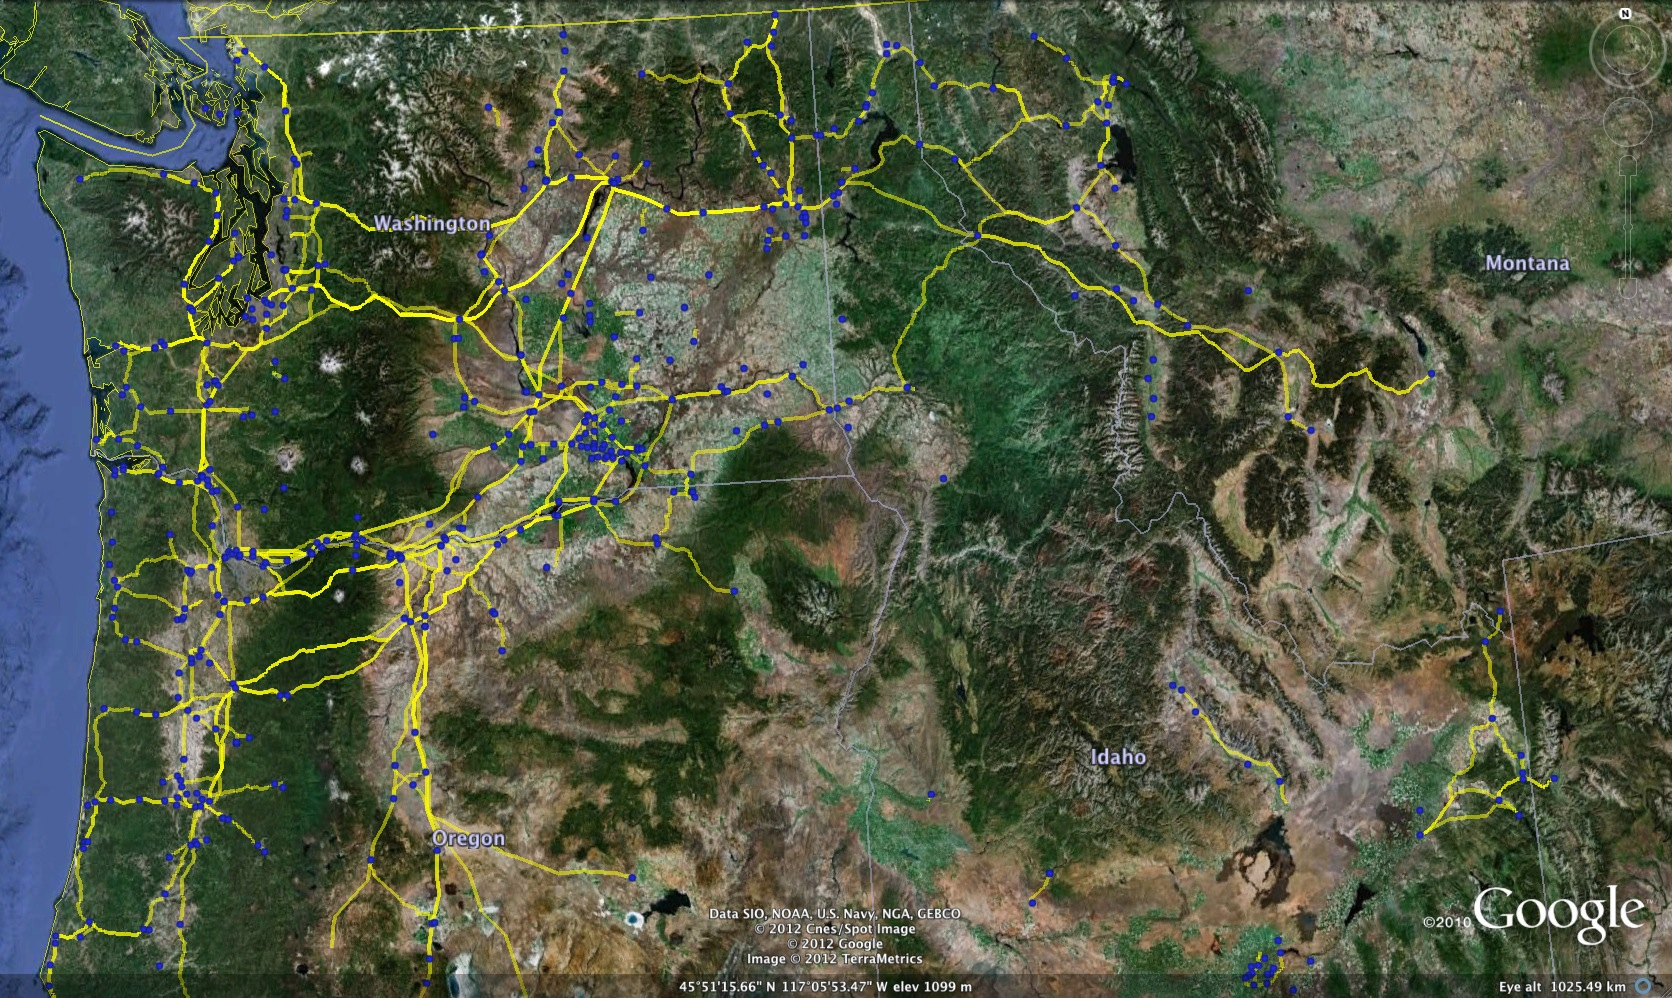
\includegraphics[scale=0.3]{BpaSystem.jpg}
\end{center}
\caption{BPA Transmission System Topology}
\end{figure}

\subsubsection {Publishers}
For the initial deployment I propose that each transmission line will have a publisher 
at either end, providing mock synchrophasor data at a maximum rate of 60 Hz.  This 
reflects the real world well from the perspective of the actual devices that are 
instrumenting the power lines and providing synchrophasor data.  From an implementation 
perspective it is simple to produce the program that produces the mock synchrophasor 
data and provides it to GridStat. I actually think we have one of these in our code 
repos.  For the substations that are owned by the distribution companies or generation 
companies, I propose that each have a single publisher that produces a synchrophasor 
that represents the low-voltage side of the substation.  This basic infrastructure 
creates enough data to be interesting in the here-and-now for conducting experimentation
 on GridStat and for later down the road when real power system simulation and control
 comes into play.  The GridStat infrastructure can be tested at the scale it is meant 
to operate at.


\subsubsection {Subscribers}
Transmission system subscribers will be broken down into two classes.  First, wide-area
 control class subscribers will subscribe to all the data in the system at relatively
 low rates, say anything less than 10 Hz.  While this may seem low it is much faster 
than rates realized by today's SCADA systems that operate of time intervals of a few 
seconds.  The second class of subscribers for the TRANSCO will be regional subscribers.
  These subscribers will operate at rates closer to the publication maximum rate of 
60 Hz, say between 30-60 Hz.  The goal of these subscribers is to reflect the needs of
 regional controllers and state-estimators within the system.  An example of this from 
the PAC realm could be a controller running an algorithm to protect a system of 
transmission lines running between a few substations.  From the SCADA realm, there is 
active research currently happening on hierarchical state estimation at WSU that uses 
a similar approach with regional state estimators feeding a global state estimator to
 produce a global snapshot of the system.  This approach not only reduces 
communications overhead, but also nicely distributes the computational overhead of the
 state estimation algorithm itself.   The TRANSCO will also subscribe to DISTCO and 
GENCO publishers at a rate similar to the SCADA rate to keep track of load and 
generation characteristics.  This will also help to flesh out some interesting 
details in federation policies between brokers.\\

From the distribution and generation side of things, each owning entity would subscribe 
to the publishers at each of its substations at variable rates.  These entities would
 also subscribe to a small number of its nearest neighbor TRANSCO substations.  
I am not sure about the electrical motivations for this, however, from a 
communications standpoint, it provides a fault-tolerance mechanism for the DISTCO's 
and GENCO's with respect to the TRANSCO's.  If for some reason a data stream fails 
from one TRANSCO forwarding engine to the DISTCO or GENCO it can resort to a nearest 
neighbor.


\subsubsection{Data and Management Planes}
As stated before the management plane will be partitioned as a QoS-Broker per owning 
entity, totaling in 117 brokers.  This will be a scale never before tested for the
 management plane.  Each QoS-Broker will be set up with a standard policy based on
 whether it is a TRANSCO broker or a DISTCO/GENCO broker.  TRANSCO brokers and 
DISTCO/GENCO brokers will have to federate with one another in well defined ways.  
The policies set in place for each must allow the DISTCO/GENCO to acquire streams 
from the TRANSCO, while providing the TRANSCO with facilities to reject subscription
 requests from DISTCO/GENCO for information that it is not allowed to access.  There 
is an analogous situation in the opposite direction from subscriptions propagating from 
the TRANSCO to the DISTCO/GENCO. \\

For the data plane, the publishers and subscribers are obviously co-located with their
 publishing and subscribing devices or applications.  For forwarding engines we will
 select a set of substations along major transmission paths (500 kV and maybe 230 kV)
 to host forwarding engines.  On the distribution and generation side, since we are not
 really representing these systems except for their connecting point with the 
transmission system they will just contain a single forwarding engine for each 
substation they own.


\subsection{Implications}
The deployment of the proposed GridStat implementation on DETER would allow for both 
scalability and security experimentation at a scale not seen before, specifically with
 the management plane.  Tight management of the interactions with QoS-Brokers is
 very important for the potential users of GridStat. Security is of paramount concern 
here.  A malicious broker or attacks on the management plane can have detrimental 
effects on the GridStat system.  The DETER testbed provides an optimal environment to 
experiment with mechanisms engineered to defend against such circumstances at a scale 
that reflects the real target operating environment. \\

Although the 'electrical infrastructure' proposed is high level and simple, I think 
that it provides a good first top-down step toward total system representation. 
Applications including state estimation are possible at this high level.  As 
research and development evolves in scalable power system simulation, this element 
can be incorporated into the framework along with the control systems that operate
over it facilitated by the GridStat communications system.



\end{document}